%\newpage
\section{Convolutional Neural Networks}

This section introduces a specific class of neural networks that has been shown very effective in processing images. 
%
In 1998, Yann LeCun and his collaborators developed a neural network for handwritten digits called LeNet \cite{726791}. It is a feedforward network with several hidden layers, trained with the backpropagation algorithm. It is later formalised with the name  convolutional neural networks (CNNs). Since LeNet, there are many other variants of CNNs, such as AlexNet, VGG16, ResNet, GoogLeNet, and so on. These variants introduce new functional layers or training methods that help improve the performance of the CNNs in pattern recognition tasks. 


\begin{figure}[!htbp]
    \centering
    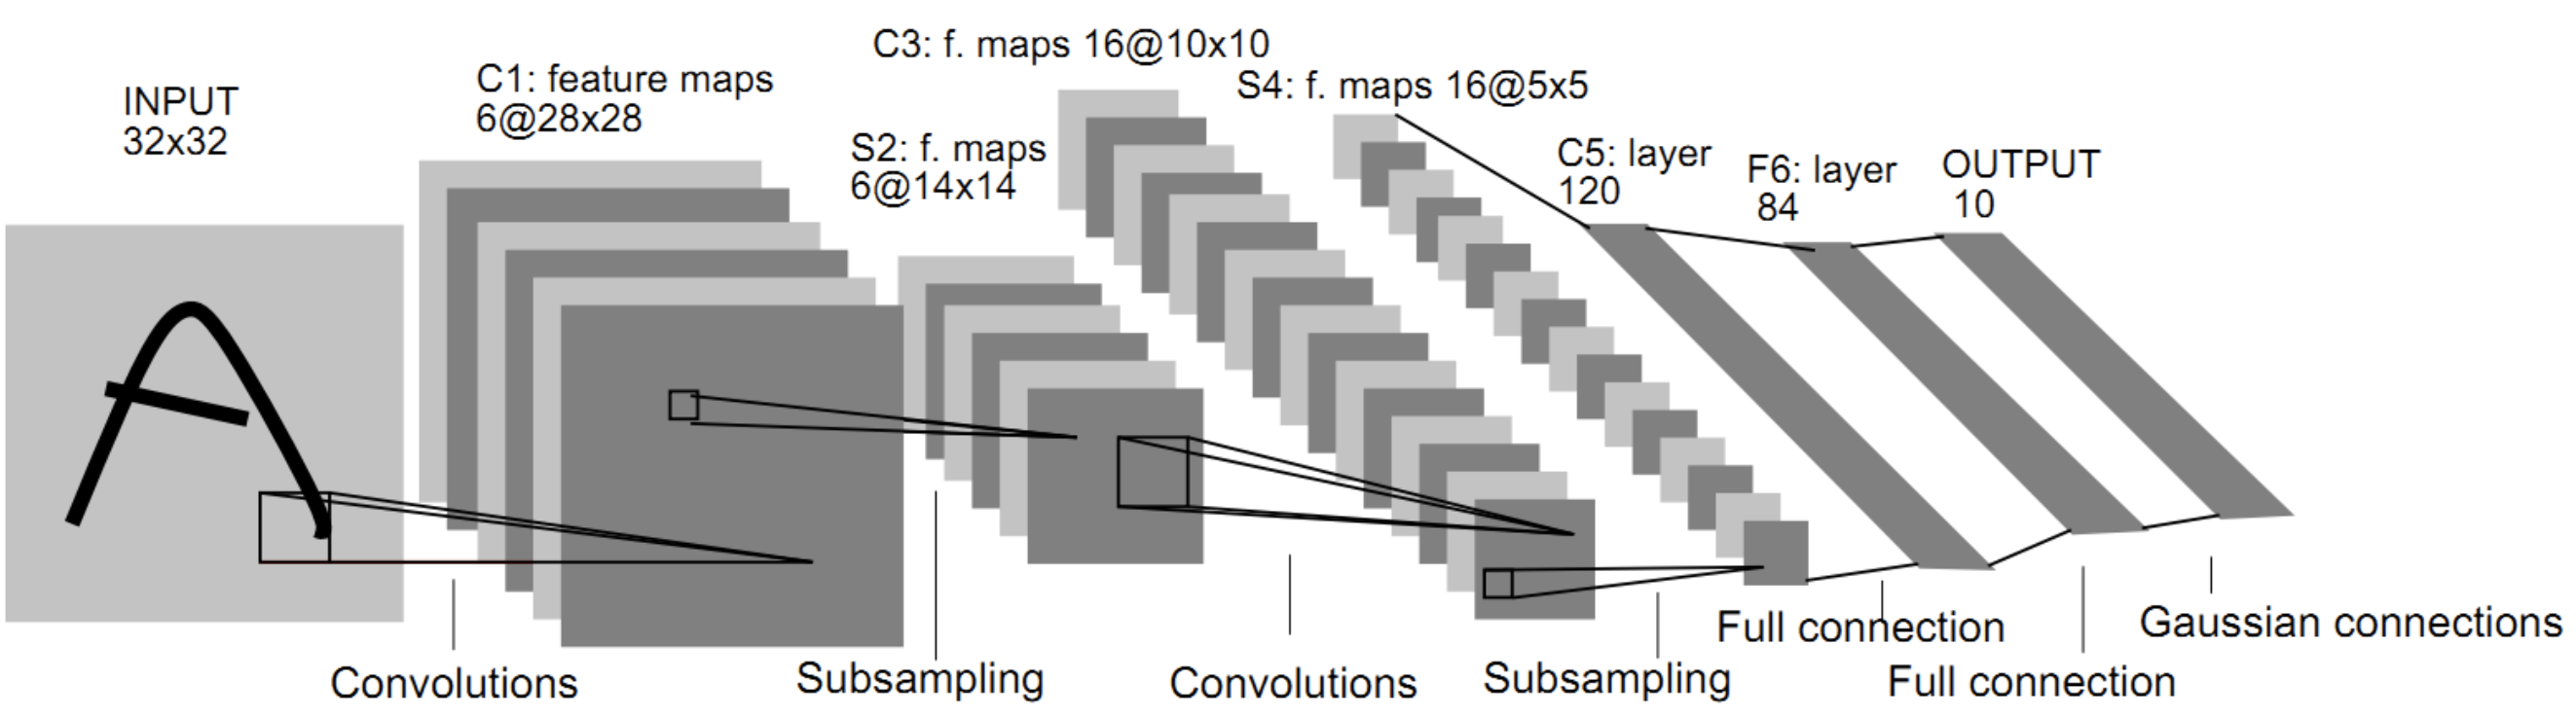
\includegraphics[width=\textwidth]{images/deepLearning/CNN/LeNet.png}
    \caption{Architecture of LeNet-5 \cite{726791}, a convolutional neural network for digits recognition. }
    \label{fig:LeNet}
\end{figure}


As shown in Figure~\ref{fig:LeNet}, LeNet has an input layer, 6 hidden layers, and an output layer. Among the 4 hidden layers, there are 2 convolutional layers, 2 subsampling (or pooling) layers, and 2 fully connected layers. 
%
Actually, common functional layers of a CNN can be e.g., fully-connected layers, convolutional layers, pooling layers, etc. It is very often that a functional layer is followed by an activation layer, such as ReLU layer, Sigmoid layer, Tanh layer, etc. After a sequence of functional and activation layers, we need a softmax layer to convert the output into a probability distribution. 

In the following, we first introduce functional layers, activation functions, and softmax layer that have been widely used in various CNNs, and then present a few common practices that have been used to either prepare data for training in or support the training. 



\subsection{Functional Layers}\label{sec:functionallayers}

As suggested earlier, each layer function $f_i$ is a mapping from a high-dimensional space $\real^{k_{i-1}}$ (that associates with Layer-$(i-1)$) to another $\real^{k_{i}}$ (that associates with Layer-$i$). That is, given $\textbf{v}_{i-1}\in \real^{k_{i}}$, we have $\textbf{v}_{i}=f_{i}(\textbf{v}_{i-1})\in \real^{k_{i}}$. 

Actually, in most CNN layers, the transformation $f_{i}$ is conducted in two steps. For the first step, it is transformed with a linear transformation, and in the second step, every neuron passes through an activation function. Formally, 
\begin{equation}
    \textbf{u}_{i}=\textbf{W}_{i}\textbf{v}_{i-1}+\textbf{b}_i \text{~~~~ and ~~~~} \textbf{v}_{i} = \sigma_i(\textbf{u}_{i})
\end{equation}
where $\sigma_i$ is an activation function. In the following, we introduce functional layers, followed by activation functions. 


\subsubsection{Fully-connected Layer}

In a fully connected layer, every neuron
receives inputs from all neurons of the previous layer, and the output of the neuron is the result of the linear combination of the inputs.  As shown in Figure~\ref{fig:fully-connected}, Layer 2 is a fully-connected layer. The neuron $n_{21}$ receives inputs from all neurons $n_{11},...,n_{16}$ in Layer 1, and weighted them with the learnable weights $\textbf{W}_{21}=(w_{21,11},...,w_{21,16})$. Therefore, its value 
\begin{equation}
    u_{21} = \textbf{W}_{21}\times \textbf{v}_1 + b_2 = w_{21,11}v_{11} + ... + w_{21,16}v_{16} + b_2
\end{equation}
where $b_2$ is the bias of layer 2. Similar for the neuron $n_{22}$. 

Note that, in the above, we use symbol $u$, instead of $v$, to denote the value of the neuron, because the output of this neuron normally needs to pass through an activation function, i.e., 
\begin{equation}
    v_{21} = \alpha(u_{21}) 
\end{equation}
We will introduce activation functions $\alpha$ later. 

\begin{figure}[!htbp]
    \centering
    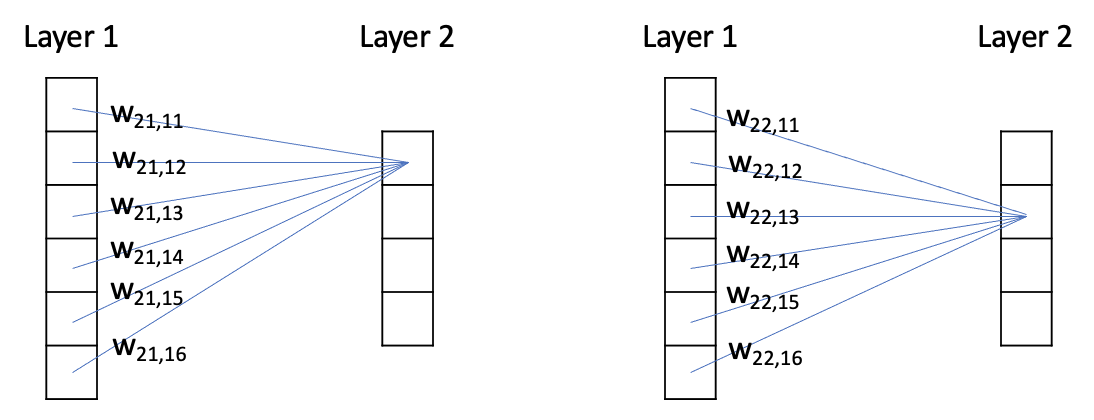
\includegraphics[width=0.7\textwidth]{images/deepLearning/CNN/fully-connected.png}
    \caption{Illustration of fully-connected layer}
    \label{fig:fully-connected}
\end{figure}

In a CNN, fully connected layers often appear in the last few layers, after the convolutional layers. The main functionality of those fully-connected layers is to implement classification over those features extracted by the convolutional layers.  
 

\subsubsection{Convolutional Layer}

Given an $n\times n$ matrix $\textbf{x}$ and an $m\times m$ filter $\textbf{f}$, we can compute the resulting matrix $\textbf{z}$ by repeatedly (1) overlapping the filter over the matrix, as illustrated in Figure~\ref{fig:convolutinallayer} with the red dashed lines,  and (2) computing an element $z_{i,j}$ with element-wise multiplication, as illustrated in Figure~\ref{fig:convolutinallayer} with the blue dashed lines.

The overlapping usually starts from the element (1,1) of the matrix $\textbf{x}$. Therefore, the (1,1) element in the resulting matrix $\textbf{z}$ is computed as follows with the element-wise multiplication: 
\begin{equation}
    z_{1,1} = \sum_{k=0}^{m-1}\sum_{l=0}^{m-1} x_{1+k,1+l}\times f_{1+k,1+l}
\end{equation}

Afterwards, it depends on a parameter $stride$ to determine the next element on $\textbf{x}$. For example, if $stride=1$, then one of the next elements, along the horizontal direction, is $(1,1+stride)= (1,2)$ such that  
\begin{equation}
    z_{1,2} = \sum_{k=0}^{m-1}\sum_{l=0}^{m-1} x_{1+k,1+l+stride}\times f_{1+k,1+l}= \sum_{k=0}^{m-1}\sum_{l=0}^{m-1} x_{1+k,1+l+1}\times f_{1+k,1+l}
\end{equation}
The other next element, along the vertical direction, is $(1+stride,1)= (2,1)$ such that  
\begin{equation}
    z_{2,1} = \sum_{k=0}^{m-1}\sum_{l=0}^{m-1} x_{1+k+stride,1+l}\times f_{1+k,1+l}= \sum_{k=0}^{m-1}\sum_{l=0}^{m-1} x_{1+k+1,1+l}\times f_{1+k,1+l}
\end{equation}
Figure~\ref{fig:convolutinallayer} presents the case where we move horizontally with $stride=1$. 

If $stride=2$, the next horizontal  element on $\textbf{x}$ will be $(1,1+stride)=(1,3)$ and we are computing the $(1,2)$ element for the resulting matrix $\textbf{z}$, i.e., 
\begin{equation}
    z_{1,2} = \sum_{k=0}^{m-1}\sum_{l=0}^{m-1} x_{1+k,1+l+stride}\times f_{1+k,1+l}= \sum_{k=0}^{m-1}\sum_{l=0}^{m-1} x_{1+k,1+l+2}\times f_{1+k,1+l}
\end{equation}
Similarly, the next vertical  element $(2,1)$ is computed as follows: 
\begin{equation}
    z_{2,1} = \sum_{k=0}^{m-1}\sum_{l=0}^{m-1} x_{1+k+stride,1+l}\times f_{1+k,1+l}= \sum_{k=0}^{m-1}\sum_{l=0}^{m-1} x_{1+k+2,1+l}\times f_{1+k,1+l}
\end{equation}
Note that, no matter what the $stride$ is, the incremental to the element on $\textbf{z}$ is always 1, to make sure that we are constructing $\textbf{z}$ one element by one element. 


\begin{figure}[!htbp]
    \centering
    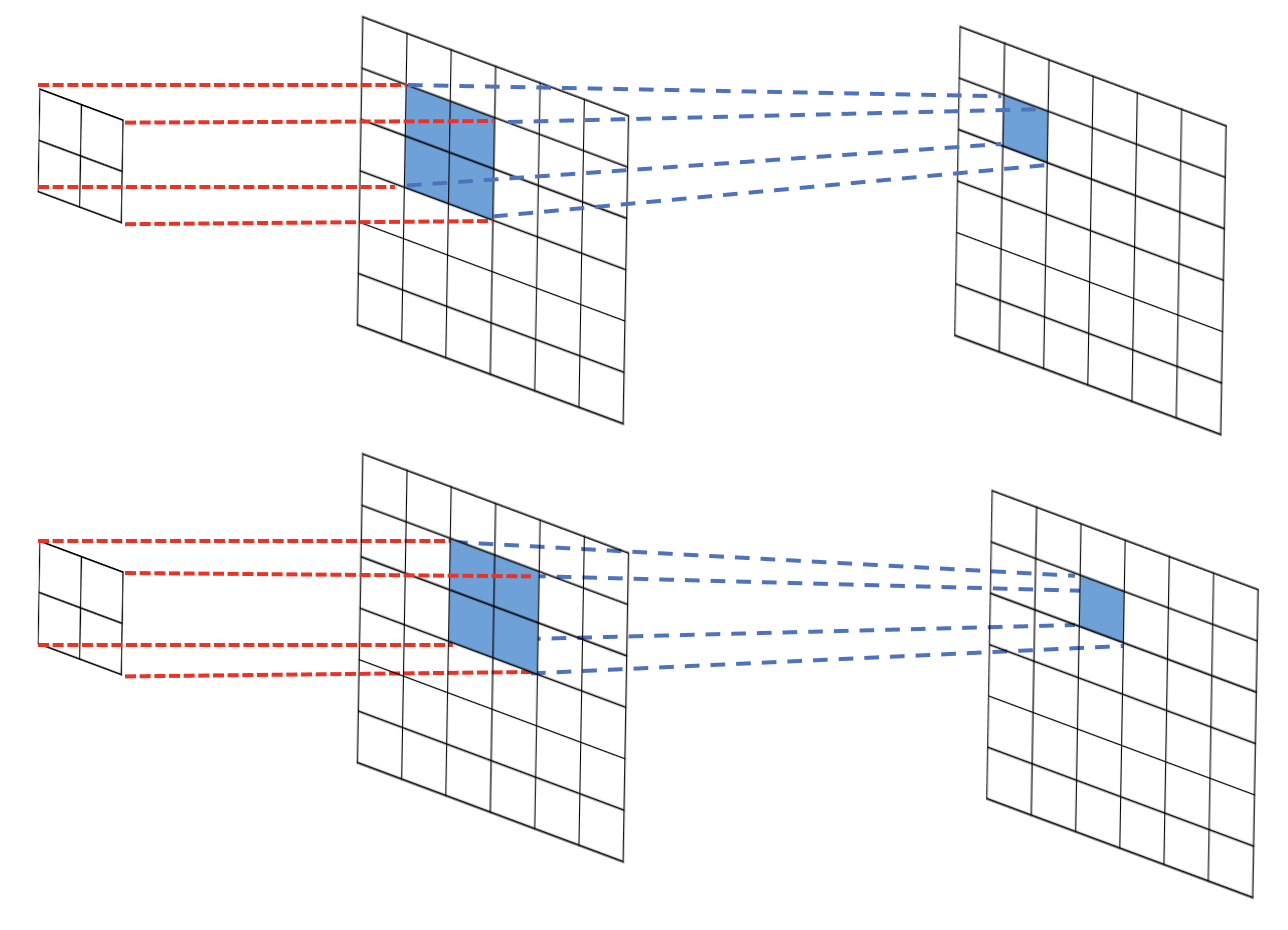
\includegraphics[width=0.9\textwidth]{images/deepLearning/CNN/convolutional.png}
    \caption{Illustration of convolutional layer}
    \label{fig:convolutinallayer}
\end{figure}

We can see that, $\textbf{z}$ is a $t\times t$ matrix such that 
\begin{equation}
    t = \frac{n-m}{stride}+1
\end{equation}
For example, if $n=4$ and $m=2$, then $t=3$ when $stride=1$ and $t=2$ when $stride=2$. 

\subsubsection{Zero-Padding}

As we can see from the previous discussion on the convolutional layer, the shapes of the matrices $\textbf{x}$ and $\textbf{z}$ are not the same. It is possible that we might be interested in maintaining the shape of the matrix along a sequence of convolutional operations. In this case, it is useful to consider a pre-processing on $\textbf{x}$ before the convolutional filter is applied. 
%
Zero-padding, a typical pre-processing operation, is to use 0 to pad the input with 0-cells, as shown in Figure~\ref{fig:zeropadding}. 

\begin{figure}
    \centering
    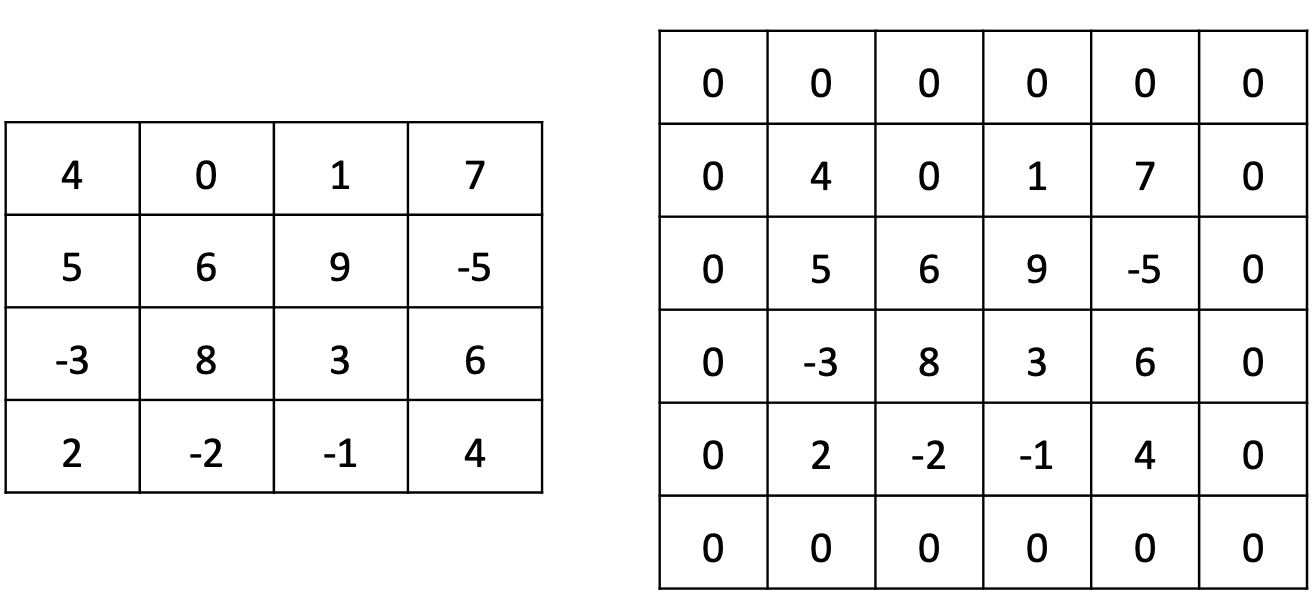
\includegraphics[width=0.6\textwidth]{images/deepLearning/CNN/padding.png}
    \caption{Zero-padding: pad the input with 0-cells around it. }
    \label{fig:zeropadding}
\end{figure}

We can see that,  if we pad $\textbf{x}$ with a border of $u$ zero valued pixels, $\textbf{z}$ is a $t\times t$ matrix such that 
\begin{equation}
    t = \frac{n-m+2*u}{stride}+1
\end{equation}
In Figure~\ref{fig:zeropadding}, $u=1$. Therefore, if $n=4$ and $m=2$ and $u=1$, then $t=5$ when $stride=1$ and $t=3$ when $stride=2$. 

\subsubsection{Pooling Layer}

A pooling layer is to reduce the information in a matrix by collapsing elements with operations. The pooling layer is frequently used in convolutional neural networks with the purpose of progressively reducing the spatial size of the representation to reduce the number of features and the computational complexity of the network. Assume that, as shown in Figure~\ref{fig:maxpooling}, we have a $4\times 4$ matrix. An application of a $2\times 2$ max-pooling filter, under the condition that $stride = 2$, will get a $2\times 2$ matrix by collapsing every $2\times 2$ block with the $\max$ operation. 

 
 
 \begin{figure}
    \centering
    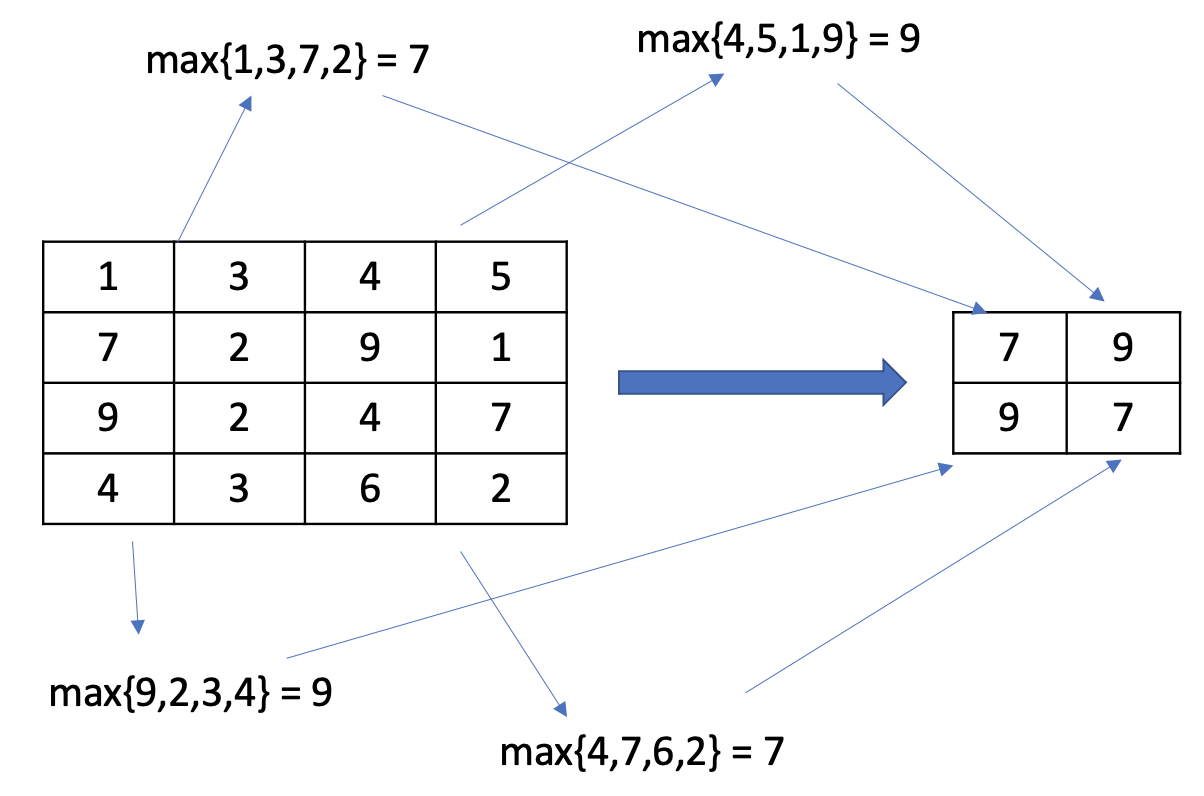
\includegraphics[width=0.6\textwidth]{images/deepLearning/CNN/maxpooling.png}
    \caption{Max-pooling. An application of $2\times 2$ filter, $stride=2$, on a $4\times 4$ matrix.}
    \label{fig:maxpooling}
\end{figure}

In addition to max-pooling, there are other pooling layers, such as the average-pooling layer, which replaces the $\max$ operation with the average operation. 


\subsection{Activation Functions}

As mentioned earlier, for most functional layers, they are followed by an activation layer where 

\subsection*{ReLU}

\begin{equation}
    ReLU(x) = max(0,x)
\end{equation}

\subsection*{Sigmoid}

\begin{equation}
    \sigma(x) = \frac{1}{1+e^{-x}}
\end{equation}
such that $\sigma'(x)=\sigma(x)(1-\sigma(x))$. 

\subsection*{Softmax}

\begin{equation}
    \delta(\textbf{v}) = (\frac{e^{v_1}}{\sum_{i=1}^{|\textbf{v}|}e^{v_i}},...,\frac{e^{v_{|\textbf{v}|}}}{\sum_{i=1}^{|\textbf{v}|}e^{v_i}}) 
\end{equation}

\subsection{Data Preprocessing}\label{sec:dataprocessing}

A suitable pre-processing of the training data can have a significant impact on the performance of the resulting model. In the following, we introduce a few different data pre-processing methods. Whether or not a specific pre-processing method should be applied is problem-specific, depending on the dataset and the machine learning task. 

\subsection*{Mean normalization} removes the mean from each data sample, i.e., 
\begin{equation}
    \textbf{x}'=\textbf{x}-\bar{\textbf{x}}
\end{equation}
where $\displaystyle\bar{\textbf{x}}=\frac{1}{|D|}\sum_{\textbf{x}\in D}\textbf{x}$ is the mean of the dataset $D$. 


\subsection*{Standardization or normalization} requires, on top of the mean normalisation, all features to be on the same scale, i.e., every sample $\textbf{x}$ is converted into 
\begin{equation}
    \textbf{x}'=\frac{\textbf{x}-\bar{\textbf{x}}}{\sigma_D}
\end{equation}
where $\sigma_D$ is the standard deviation of the dataset $D$.

\subsection*{Whitening} requires that the covariance matrix of the converted dataset is the identity matrix -- 1 in the diagonal and 0 for the other cells. It first applies the mean normalisation on the dataset $D$ to get $D'$, and then apply a whitening matrix $W$ on every sample, i.e., let $\textbf{x}''=\textbf{W}\textbf{x}'$, such that $\textbf{W}\textbf{W}^T=\Sigma^{-1}$ and $\Sigma$ is the non-singular covariance matrix of $D'$.

Depending on what $\textbf{W}$ is, we have Mahalanobis or ZCA whitening ($\textbf{W}=\Sigma^{-1/2}$), Cholesky whitening ($\textbf{W}=\textbf{L}^T$ for $\textbf{L}$ the  Cholesky decomposition of $\Sigma^{-1}$), or PCA whitening ($\textbf{W}$ is the eigen-system of $\Sigma^{-1}$).  

\subsection{Practice}

%[xiaowei: here we need a code piece to train a convolutional neural networks and retrieve the weights. ]

First, we setup hyper-parameters (e.g., batchsize, epoch, learning rate), device (e.g., CPU or GPU), and load training dataset (MNIST).
\begin{lstlisting}[language=Python]
import torch
import torch.nn as nn
import torch.nn.functional as F
import torch.optim as optim
from torchvision import datasets, transforms
import argparse
import time
import os

# Setup training parameters
parser = argparse.ArgumentParser(description='PyTorch MNIST Training')
parser.add_argument('--batch-size', type=int, default=128, metavar='N',
                    help='input batch size for training (default: 128)')
parser.add_argument('--test-batch-size', type=int, default=128, metavar='N',
                    help='input batch size for testing (default: 128)')
parser.add_argument('--epochs', type=int, default=5, metavar='N',
                    help='number of epochs to train')
parser.add_argument('--lr', type=float, default=0.01, metavar='LR',
                    help='learning rate')
parser.add_argument('--no-cuda', action='store_true', default=False,
                    help='disables CUDA training')
parser.add_argument('--seed', type=int, default=1, metavar='S',
                    help='random seed (default: 1)')
parser.add_argument('--model-dir', default='./model-mnist-cnn',
                    help='directory of model for saving checkpoint')
parser.add_argument('--load-model', action='store_true', default=False,
                    help='load model or not')

args = parser.parse_args(args=[]) 

if not os.path.exists(args.model_dir):
    os.makedirs(args.model_dir)
        
# Judge cuda is available or not
use_cuda = not args.no_cuda and torch.cuda.is_available()
#device = torch.device("cuda" if use_cuda else "cpu")
device = torch.device("cpu")

torch.manual_seed(args.seed)
kwargs = {'num_workers': 1, 'pin_memory': True} if use_cuda else {}

# Setup data loader
transform=transforms.Compose([
        transforms.ToTensor(),
        transforms.Normalize((0.1307,), (0.3081,))
        ])
trainset = datasets.MNIST('../data', train=True, download=True,
                   transform=transform)
testset = datasets.MNIST('../data', train=False,
                   transform=transform)
train_loader = torch.utils.data.DataLoader(trainset,batch_size=args.batch_size, shuffle=True,**kwargs)
test_loader = torch.utils.data.DataLoader(testset,batch_size=args.test_batch_size, shuffle=False, **kwargs)
\end{lstlisting}

We can define a convolutional neural network as follows, with 2 convolutional layers and 2 fully connected layers.
\begin{lstlisting}[language=Python]
# Define CNN
class Net(nn.Module):
    def __init__(self):
        super(Net, self).__init__()
        # in_channels:1  out_channels:32  kernel_size:3  stride:1
        self.conv1 = nn.Conv2d(1, 32, 3, 1)
        # in_channels:32  out_channels:64  kernel_size:3  stride:1
        self.conv2 = nn.Conv2d(32, 64, 3, 1)
        self.fc1 = nn.Linear(9216, 128)
        self.fc2 = nn.Linear(128, 10)

    def forward(self, x):
        x = self.conv1(x)
        x = F.relu(x)
        x = self.conv2(x)
        x = F.relu(x)
        x = F.max_pool2d(x, 2)
        x = torch.flatten(x, 1)
        x = self.fc1(x)
        x = F.relu(x)
        x = self.fc2(x)
        output = F.log_softmax(x, dim=1)
        return output
\end{lstlisting}

\begin{lstlisting}[language=Python]
# Train function
def train(args, model, device, train_loader, optimizer, epoch):
    model.train()
    for batch_idx, (data, target) in enumerate(train_loader):
        data, target = data.to(device), target.to(device)
        
        #clear gradients
        optimizer.zero_grad()
        
        #compute loss
        loss = F.cross_entropy(model(data), target)
        
        #get gradients and update
        loss.backward()
        optimizer.step()
        
# Predict function
def eval_test(model, device, test_loader):
    model.eval()
    test_loss = 0
    correct = 0
    with torch.no_grad():
        for data, target in test_loader:
            data, target = data.to(device), target.to(device)
            output = model(data)
            test_loss += F.cross_entropy(output, target, size_average=False).item()
            pred = output.max(1, keepdim=True)[1]
            correct += pred.eq(target.view_as(pred)).sum().item()
    test_loss /= len(test_loader.dataset)
    test_accuracy = correct / len(test_loader.dataset)
    return test_loss, test_accuracy
\end{lstlisting}

Finally, we define the main function, which can load the trained model, or train the initial model and save the trained model.
\begin{lstlisting}[language=Python]
# Main function, train the initial model or load the model
def main():
    model = Net().to(device)
    optimizer = optim.SGD(model.parameters(), lr=args.lr)
    
    if args.load_model:
        # Load model
        model.load_state_dict(torch.load(os.path.join(args.model_dir, 'final_model.pt')))
        trnloss, trnacc = eval_test(model, device, train_loader)
        tstloss, tstacc = eval_test(model, device, test_loader)
        print('trn_loss: {:.4f}, trn_acc: {:.2f}%'.format(trnloss, 100. * trnacc), end=', ')
        print('test_loss: {:.4f}, test_acc: {:.2f}%'.format(tstloss, 100. * tstacc))
        
    else:
        # Train initial model
        for epoch in range(1, args.epochs + 1):
            start_time = time.time()

            #training
            train(args, model, device, train_loader, optimizer, epoch)

            #get trnloss and testloss
            trnloss, trnacc = eval_test(model, device, train_loader)
            tstloss, tstacc = eval_test(model, device, test_loader)

            #print trnloss and testloss
            print('Epoch '+str(epoch)+': '+str(int(time.time()-start_time))+'s', end=', ')
            print('trn_loss: {:.4f}, trn_acc: {:.2f}%'.format(trnloss, 100. * trnacc), end=', ')
            print('test_loss: {:.4f}, test_acc: {:.2f}%'.format(tstloss, 100. * tstacc))
        
        #save model
        torch.save(model.state_dict(), os.path.join(args.model_dir, 'final_model.pt'))

if __name__ == '__main__':
    main()
\end{lstlisting}